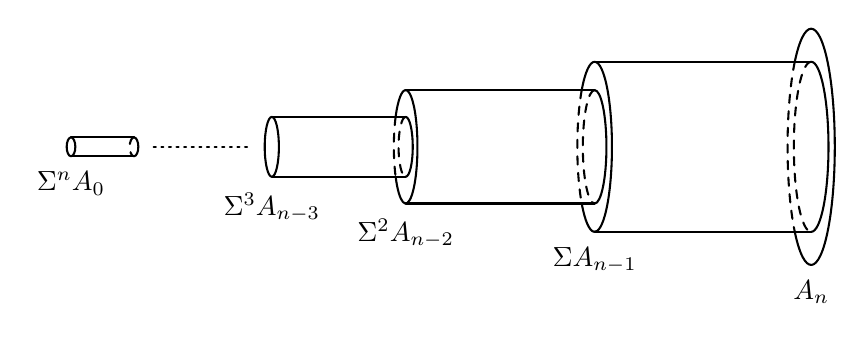
\begin{tikzpicture}[x=1cm,y=1cm,line width=.75pt,
                    line cap=round,line join=round]
  % Las dos primeras tapas izquierdas son completamente visibles.
  \def\tapaVisible#1#2#3{%
    \draw (#1,0) ellipse [x radius=#2,y radius=#3];%
  }
  % Tapa derecha: su mitad izquierda queda oculta.
  \def\tapaDerecha#1#2#3{%
    \draw[dashed] (#1,#3)
      arc[start angle=90,end angle=270,x radius=#2,y radius=#3];
    \draw (#1,#3)
      arc[start angle=90,end angle=-90,x radius=#2,y radius=#3];%
  }
  % Tapa izquierda: solo se oculta el arco comprendido entre
  % las paredes y=+#4 e y=-#4 del cilindro anterior.
  \def\tapaIzquierda#1#2#3#4{%
    \pgfmathsetmacro{\anguloOculto}{asin(#4/#3)}%
    \draw (#1,#3)
      arc[start angle=90,end angle={180-\anguloOculto},
          x radius=#2,y radius=#3];
    \draw[dashed] ({#1-#2*cos(\anguloOculto)},{#4})
      arc[start angle={180-\anguloOculto},end angle={180+\anguloOculto},
          x radius=#2,y radius=#3];
    \draw ({#1-#2*cos(\anguloOculto)},{-#4})
      arc[start angle={180+\anguloOculto},end angle=450,
          x radius=#2,y radius=#3];%
  }

  \draw (0,.12) -- (.80,.12) (0,-.12) -- (.80,-.12);
  \tapaVisible{0}{.055}{.12}
  \tapaDerecha{.80}{.055}{.12}
  \node[below=2pt] at (0,-.12) {$\Sigma^{n}A_0$};
  \draw[dotted] (1.05,0) -- (2.30,0);

  \draw (2.55,.38) -- (4.25,.38)
        (2.55,-.38) -- (4.25,-.38);
  \tapaVisible{2.55}{.09}{.38}
  \tapaDerecha{4.25}{.09}{.38}
  \node[below=2pt] at (2.55,-.38) {$\Sigma^3A_{n-3}$};

  \draw (4.25,.72) -- (6.65,.72)
        (4.25,-.72) -- (6.65,-.72);
  \tapaIzquierda{4.25}{.15}{.72}{.38}
  \tapaDerecha{6.65}{.15}{.72}
  \node[below=2pt] at (4.25,-.72) {$\Sigma^2A_{n-2}$};

  \draw (6.65,1.08) -- (9.40,1.08)
        (6.65,-1.08) -- (9.40,-1.08);
  \tapaIzquierda{6.65}{.22}{1.08}{.72}
  \tapaDerecha{9.40}{.22}{1.08}
  \node[below=2pt] at (6.65,-1.08) {$\Sigma A_{n-1}$};

  \tapaIzquierda{9.40}{.30}{1.50}{1.08}
  \node[below=2pt] at (9.40,-1.50) {$A_{n}$};
\end{tikzpicture}